\documentclass[sigplan,10pt]{acmart}

\usepackage[utf8]{inputenc}
\usepackage{listings}
\usepackage{todonotes}
\usepackage{comment}    % comments.
\usepackage{url}    % url.

\settopmatter{printfolios=true}

\graphicspath{{./data/img/}}

% Copyright
%\setcopyright{none}
%\setcopyright{acmcopyright}
%\setcopyright{acmlicensed}
\setcopyright{rightsretained}
%\setcopyright{usgov}
%\setcopyright{usgovmixed}
%\setcopyright{cagov}
%\setcopyright{cagovmixed}


% DOI
%\acmDOI{10.475/123_4}

% ISBN
%\acmISBN{123-4567-24-567/08/06}

%Conference
\acmConference[SEPS 2017]{4th International Workshop on Software Engineering for Parallel Systems}{October 2017}{Vancouver, Canada}
\acmYear{2017}
\copyrightyear{2017}

%\acmPrice{15.00}

%\acmBadgeL[http://ctuning.org/ae/ppopp2016.html]{ae-logo}
%\acmBadgeR[http://ctuning.org/ae/ppopp2016.html]{ae-logo}



\begin{document}
%---
\title{A Software Engineering Perspective on \\ OpenMP and PThreads}
%\titlenote{...}
\subtitle{from the learning aspects to the real performance results}
%\subtitlenote{...}
%---
\author{Pedro Bruel}
%\authornote{This author is the one who did all the really hard work.}
\affiliation{%
  \institution{Software Systems Laboratory (LSS)\\ Institute of Mathematics and Statistics\\ University of São Paulo}
  \streetaddress{Rua do Matão, 1010}
  \city{São Paulo}
  \country{Brazil}
  \postcode{05508-090}
}
\email{phrb@ime.usp.br}
%---
\author{Paulo Meirelles}
%\authornote{Posdoc}
\affiliation{%
  \institution{FLOSS Competence Center (CCSL)\\ Institute of Mathematics and Statistics\\ University of São Paulo}
  \streetaddress{Rua do Matão, 1010}
  \city{São Paulo}
  \country{Brazil}
  \postcode{05508-090}
}
\email{paulormm@ime.usp.br}
%---
\author{Alfredo Goldman}
%\authornote{Professor: the head.}
\affiliation{%
  \institution{Software Systems Laboratory (LSS)\\ Institute of Mathematics and Statistics\\ University of São Paulo}
  \streetaddress{Rua do Matão, 1010}
  \city{São Paulo}
  \country{Brazil}
  \postcode{05508-090}
}
\email{gold@ime.usp.br}

%---

\renewcommand{\shortauthors}{Bruel et al.}

%--
\begin{abstract}
TO-DO ...
\end{abstract}

%---

\maketitle

%---
\section{Introduction}
\label{sec:introduction}

...

In this context, the approach of using Compilation Directives to guide the
compiler in the parallelization process has gained popularity. These directives
are implemented using the compiler's pre-processing directives and are utilized
as annotations that provide tips about the sequential code. Among the tools and
extensions that use compilation directives are the \texttt{OpenMP} API
\cite{Dagum1998a} \cite{Chapman:2007} used for writing programs for multi-core
architectures, and the \texttt{OpenACC} programming
standard~\cite{openacc:api}, used for writing programs for heterogeneous
CPU/GPU architectures. The \texttt{OpenMP 4.0} specification supports
offloading capabilities \cite{openmp:api:2013} such as \texttt{OpenACC} and
\texttt{AMD HSA}~\cite{amd:hsa:site}. These tools aim to make easier the task
of designing and implementing efficient and provably correct parallel
algorithms. However, the abstraction layers built by the extensions also have
the potential to conceal architectural details and to generate new parallel
programming challenges.

When comparing \texttt{OpenMP} to other available tools for developing
multi-threaded applications such as the \texttt{pthreads} interface, the API
can be considered almost costless. However, when writing more complex
applications this may not be true. The design and implementation of such
complex applications require more knowledge about platforms and execution
models than what can be shown by tutorials, that present high level and trivial
examples. These tutorials try to convince the user that programming with
directives is simple and easy to do, which is not always true. For instance, to
achieve good performance in some cases it is necessary to describe many
restrictions on annotations~\cite{OpenMPTasks2009}~\cite{mattson2003good}.

Krawezik and Cappello~\cite{CPE:CPE905} evidenced this difficulty by comparing
MPI and three OpenMP versions of benchmarks. The most popular use of
\texttt{OpenMP} directives is at the loop level. The programmer discovers
potentially parallel loops and annotates the code with directives starting and
closing parallel regions. Good results were obtained only when SPMD was
implemented on OpenMP, and achieving good performance required a significant
programming effort~\cite{CPE:CPE905}.

In this work we have gathered data from assignments made by graduate students
for the \emph{Introduction to Parallel and Distributed Computing} course. Among
other exercises, the students were asked to find examples of \texttt{OpenMP}
code in tutorials and official manuals that failed under special conditions.
These conditions could be created by, for example, placing barriers or forcing
racing conditions by exposing inaccurate thread management.


The rest of the paper is organized as follows. The following section discusses
related work... 


\section{Background}
\label{sec:background}

%\todo[inline,color=cyan,author=Pedro]{Cite our previous paper, making it clear that we are the authors}
%\todo[inline,color=cyan,author=Pedro]{Describe related work}
%\todo[inline,color=cyan,author=Pedro]{Describe related work since last paper}

The selection of teaching tools for Parallel and Distributed classes impacts
the development of students' abilities to solve algorithmic problems
efficiently. The importance of selecting good tools for teaching Parallel and
Distributed Computing has been increasingly important, especially since the
topic became a core component of the ACM undergraduate computer science
curricula in 2013~\cite{acmcurricula}.

Different approaches have been used to study the selection of the best level of
abstraction for teaching Parallel and Distributed programming courses.
Falcao~\cite{6565518} argues that introducing a high-level parallel programming
interface such as \textit{OpenMP} in the beginning of an undergraduate computer
science course would cause a small overhead and benefit the rest of the course.
Foley \textit{et al.}~\cite{FOLEY2017138} support the introduction of practical
learning experiences along an undergraduate course, of increasing depth as the
course progresses. They introduce OnRamp, a web application to help students
learn to write parallel code starting with practical and moving to conceptual
experiences.  Pllana \textit{et al.}~\cite{Pllana:2009} adopt a Model Driven
Development approach to develop parallel solutions using Parallel Building
Blocks. They introduce a programming environment that transforms these
high-level models in source code. The tool's goal is to hide from the students
the complexity of writing parallel code.

The approaches mentioned so far introduce tools for parallel programming before
the related concepts.  Other approaches instead consider learning software
tools as just one of the objectives of the course, and argue that their
introduction should come after the introduction of concepts of Parallel and
Distributed Computing.

In previous work~\cite{goncalves:OpenMPNotEasy} we show that teaching the
concepts of parallel programming first instead of high-level parallel
programming APIs is important, especially because the available resources and
tutorials for these APIs may contain difficult to find errors.  We listed
several sources of tutorials and hands-on materials obtained in the internet in
which undergraduate students were able to point parallel correctness
errors~\cite{SuB:2005:CMO:1892830.1892863}.

Sü\ss{} and Leopold~\cite{Leopold:userOpenMP} discuss the inability to express
all parallel solutions in tools such as \textit{OpenMP}. They used a sorting
algorithm to show that it is easy to find patterns that are difficult to
implement in \textit{OpenMP}, but can be easily implemented in lower-level
programming interfaces, such as POSIX Threads.

Adams~\cite{ADAMS201731} presented a set of patterns implemented using
\textit{Pthreads} that can help students understand aspects of parallel
programming that would be difficult to grasp using only \textit{OpenMP}
examples. His catalog also contained patterns implemented in \textit{OpenMP}.

\todo[inline,color=cyan,author=Pedro]{This last paragraph maybe fits best in
the end of the introduction}

In this paper we present data that supports the importance of composing a
curriculum for Parallel and Distributed Computing courses using low-level
programming interfaces, such as \textit{Pthreads}, as well as high-level
interfaces, such as \textit{OpenMP}.  Brown \textit{et
al.}~\cite{Brown:2010:SPC:1971681.1971689}, points that the choice of a
software tool should be only one of the topics explored during a parallel
programming course. Topics such as data structures, algorithms, software design
and parallel hardware platforms should also be explored.

\todo[inline,color=orange,author=Raphael]{Maybe we should make a better
connection between the end of this section and the next one;}

\section{Related Work}
\label{sec:relatedwork}

%\todo[inline,color=cyan,author=Pedro]{Cite our previous paper, making it clear that we are the authors}
%\todo[inline,color=cyan,author=Pedro]{Describe related work}
%\todo[inline,color=cyan,author=Pedro]{Describe related work since last paper}

The selection of teaching tools for Parallel and Distributed classes impacts
the development of students' abilities to solve algorithmic problems
efficiently. The importance of selecting good tools for teaching Parallel and
Distributed Computing has been increasingly important, especially since the
topic became a core component of the ACM undergraduate computer science
curricula in 2013~\cite{acmcurricula}.

Different approaches have been used to study the selection of the best level of
abstraction for teaching Parallel and Distributed programming courses.
Falcao~\cite{6565518} argues that introducing a high-level parallel programming
interface such as \textit{OpenMP} in the beginning of an undergraduate computer
science course would cause a small overhead and benefit the rest of the course.
Foley \textit{et al.}~\cite{FOLEY2017138} support the introduction of practical
learning experiences along an undergraduate course, of increasing depth as the
course progresses. They introduce OnRamp, a web application to help students
learn to write parallel code starting with practical and moving to conceptual
experiences.  Pllana \textit{et al.}~\cite{Pllana:2009} adopt a Model Driven
Development approach to develop parallel solutions using Parallel Building
Blocks. They introduce a programming environment that transforms these
high-level models in source code. The tool's goal is to hide from the students
the complexity of writing parallel code.

The approaches mentioned so far introduce tools for parallel programming before
the related concepts.  Other approaches instead consider learning software
tools as just one of the objectives of the course, and argue that their
introduction should come after the introduction of concepts of Parallel and
Distributed Computing.

In previous work~\cite{goncalves:OpenMPNotEasy} we show that teaching the
concepts of parallel programming first instead of high-level parallel
programming APIs is important, especially because the available resources and
tutorials for these APIs may contain difficult to find errors.  We listed
several sources of tutorials and hands-on materials obtained in the internet in
which undergraduate students were able to point parallel correctness
errors~\cite{SuB:2005:CMO:1892830.1892863}.

Sü\ss{} and Leopold~\cite{Leopold:userOpenMP} discuss the inability to express
all parallel solutions in tools such as \textit{OpenMP}. They used a sorting
algorithm to show that it is easy to find patterns that are difficult to
implement in \textit{OpenMP}, but can be easily implemented in lower-level
programming interfaces, such as POSIX Threads.

Adams~\cite{ADAMS201731} presented a set of patterns implemented using
\textit{Pthreads} that can help students understand aspects of parallel
programming that would be difficult to grasp using only \textit{OpenMP}
examples. His catalog also contained patterns implemented in \textit{OpenMP}.

\todo[inline,color=cyan,author=Pedro]{This last paragraph maybe fits best in
the end of the introduction}

In this paper we present data that supports the importance of composing a
curriculum for Parallel and Distributed Computing courses using low-level
programming interfaces, such as \textit{Pthreads}, as well as high-level
interfaces, such as \textit{OpenMP}.  Brown \textit{et
al.}~\cite{Brown:2010:SPC:1971681.1971689}, points that the choice of a
software tool should be only one of the topics explored during a parallel
programming course. Topics such as data structures, algorithms, software design
and parallel hardware platforms should also be explored.

\todo[inline,color=orange,author=Raphael]{Maybe we should make a better
connection between the end of this section and the next one;}

\section{Research Design}
\label{sec:researchdesing}

The motivation to write this paper comes from experiences on teaching. During the classes of Distributed Systems and Parallel Programming, a graduate course at University of São Paulo...

\begin{description}
\item[RQ1:] \textit{Which API is easier to learn and use according to the student perceptions?}
%
...
\item[RQ2:] \textit{Which API is better to improve the performance according to the student perceptions?}
%
...

\end{description}

\subsection{Student Background}

\begin{figure}[htpb]
    \centering
    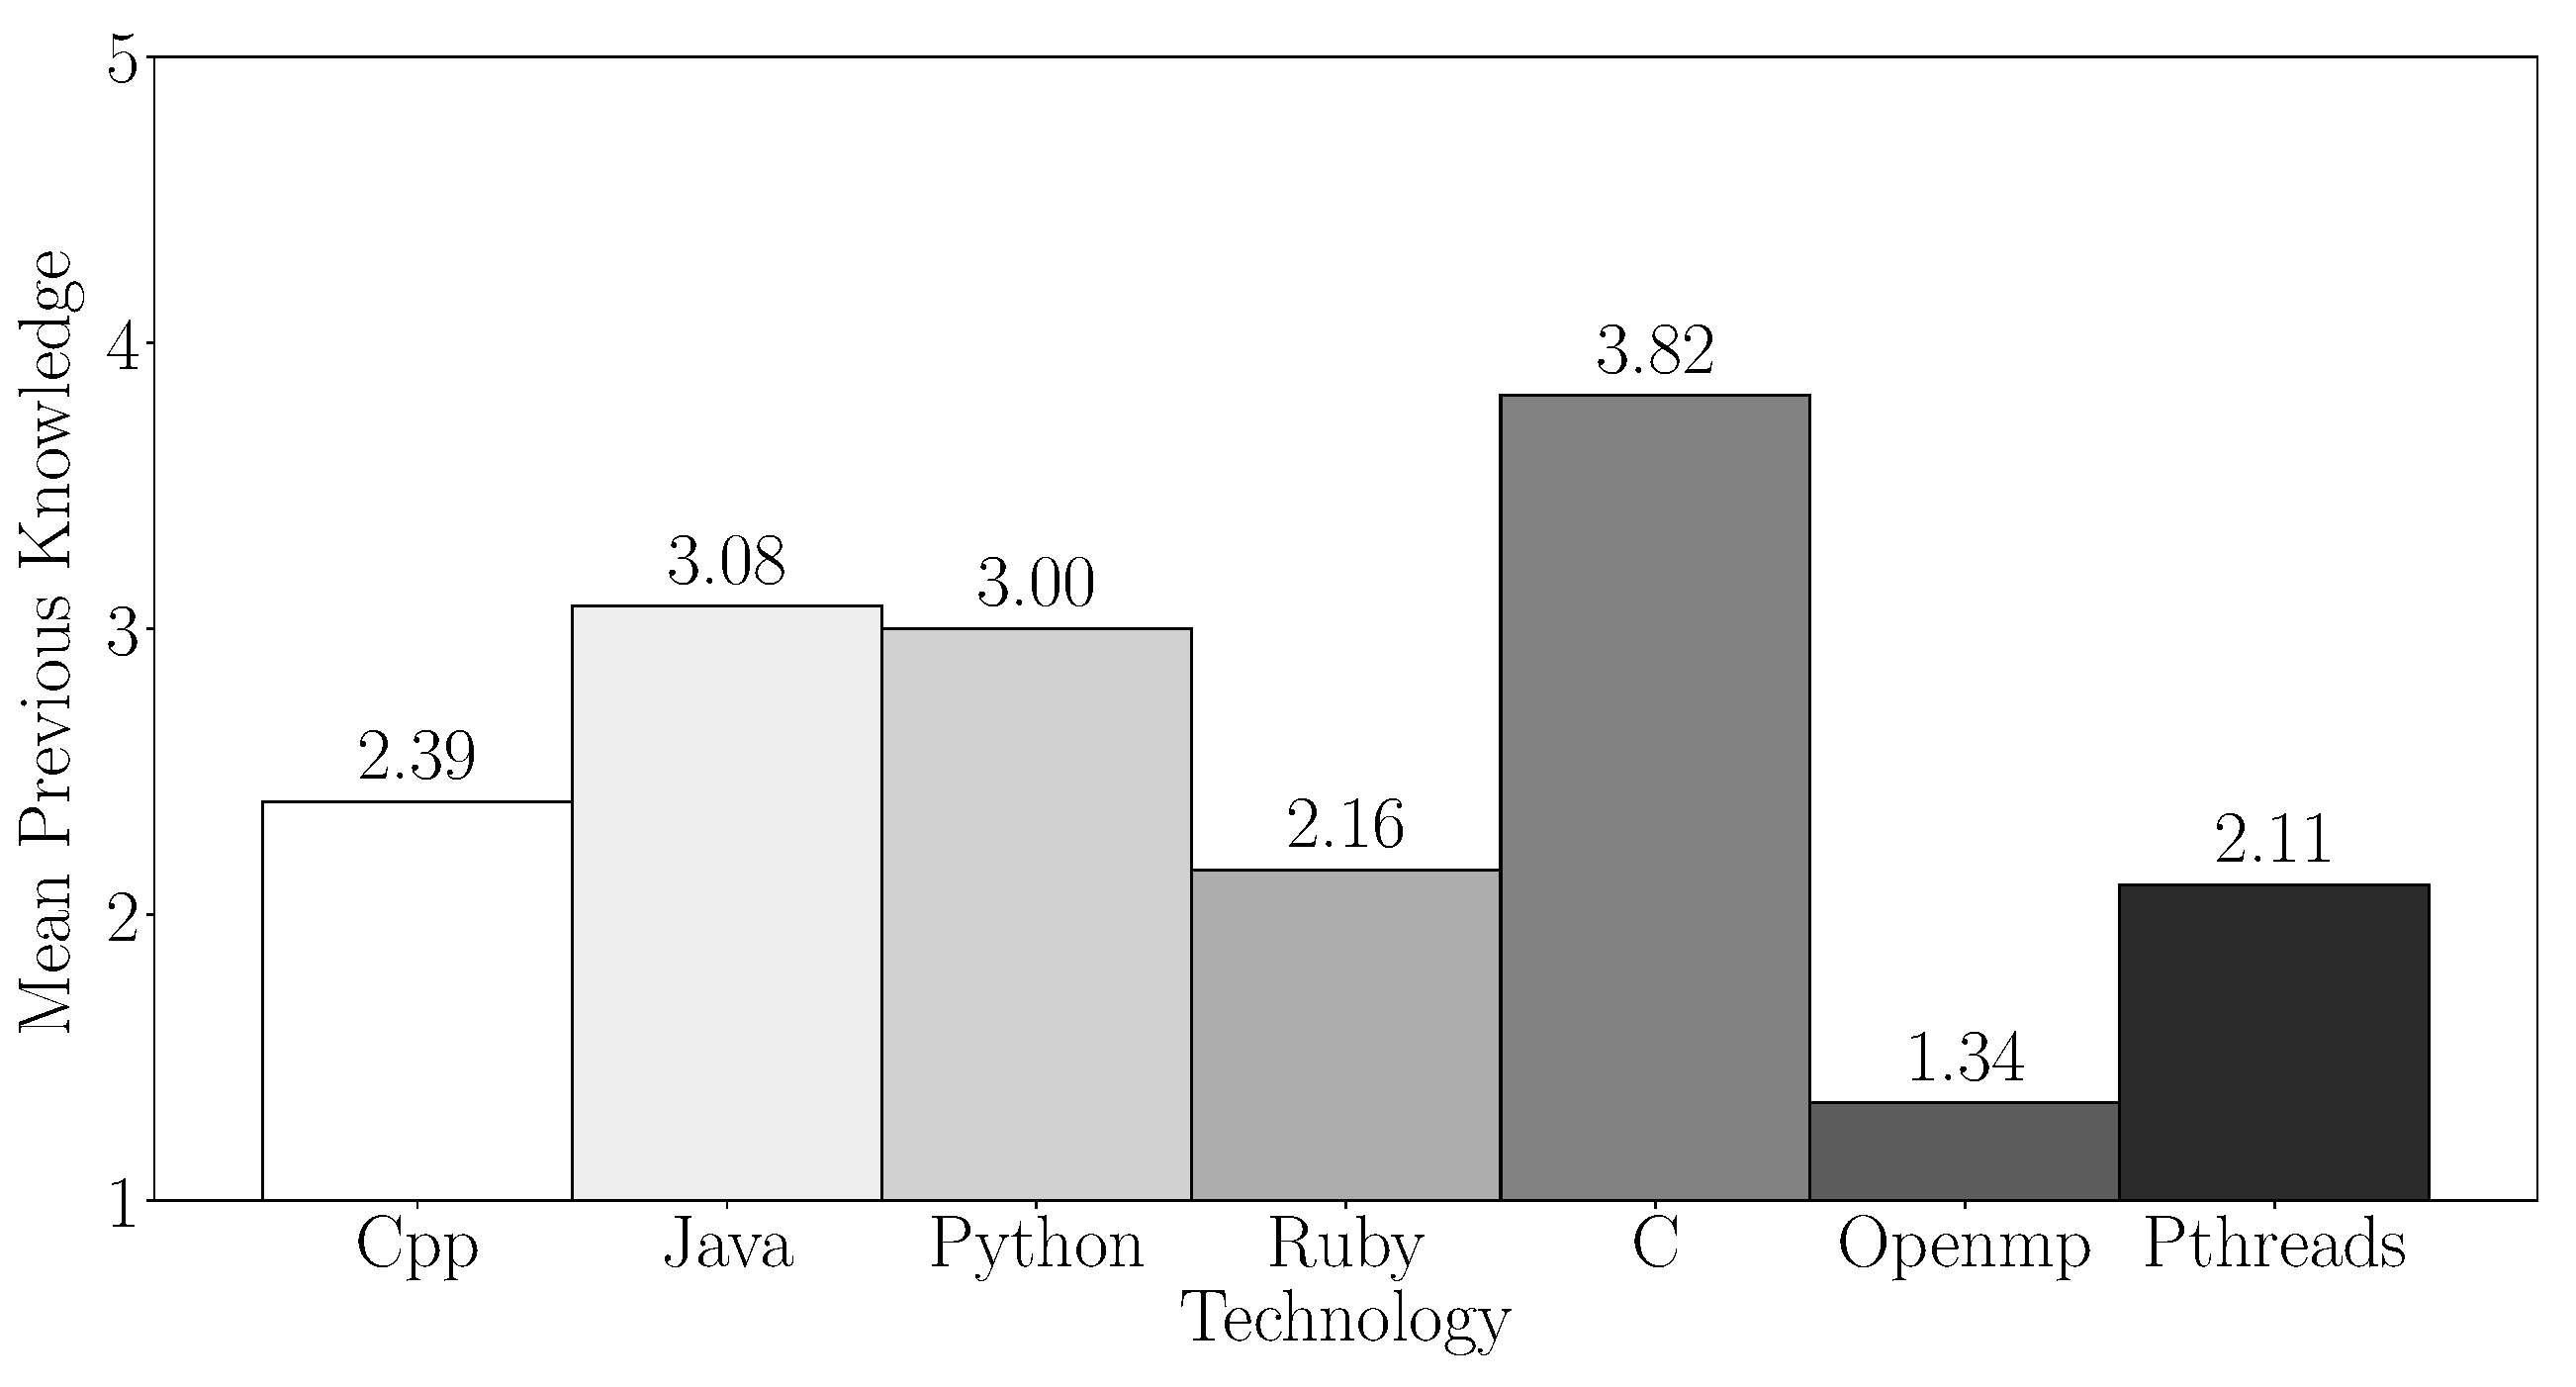
\includegraphics[width=0.85\columnwidth]{background_mean_knowledge}
    \caption{Student mean knowledge \textit{before} the assignment}
    \label{fig:student-mean-knowledge}
\end{figure}

\begin{figure}[htpb]
    \centering
    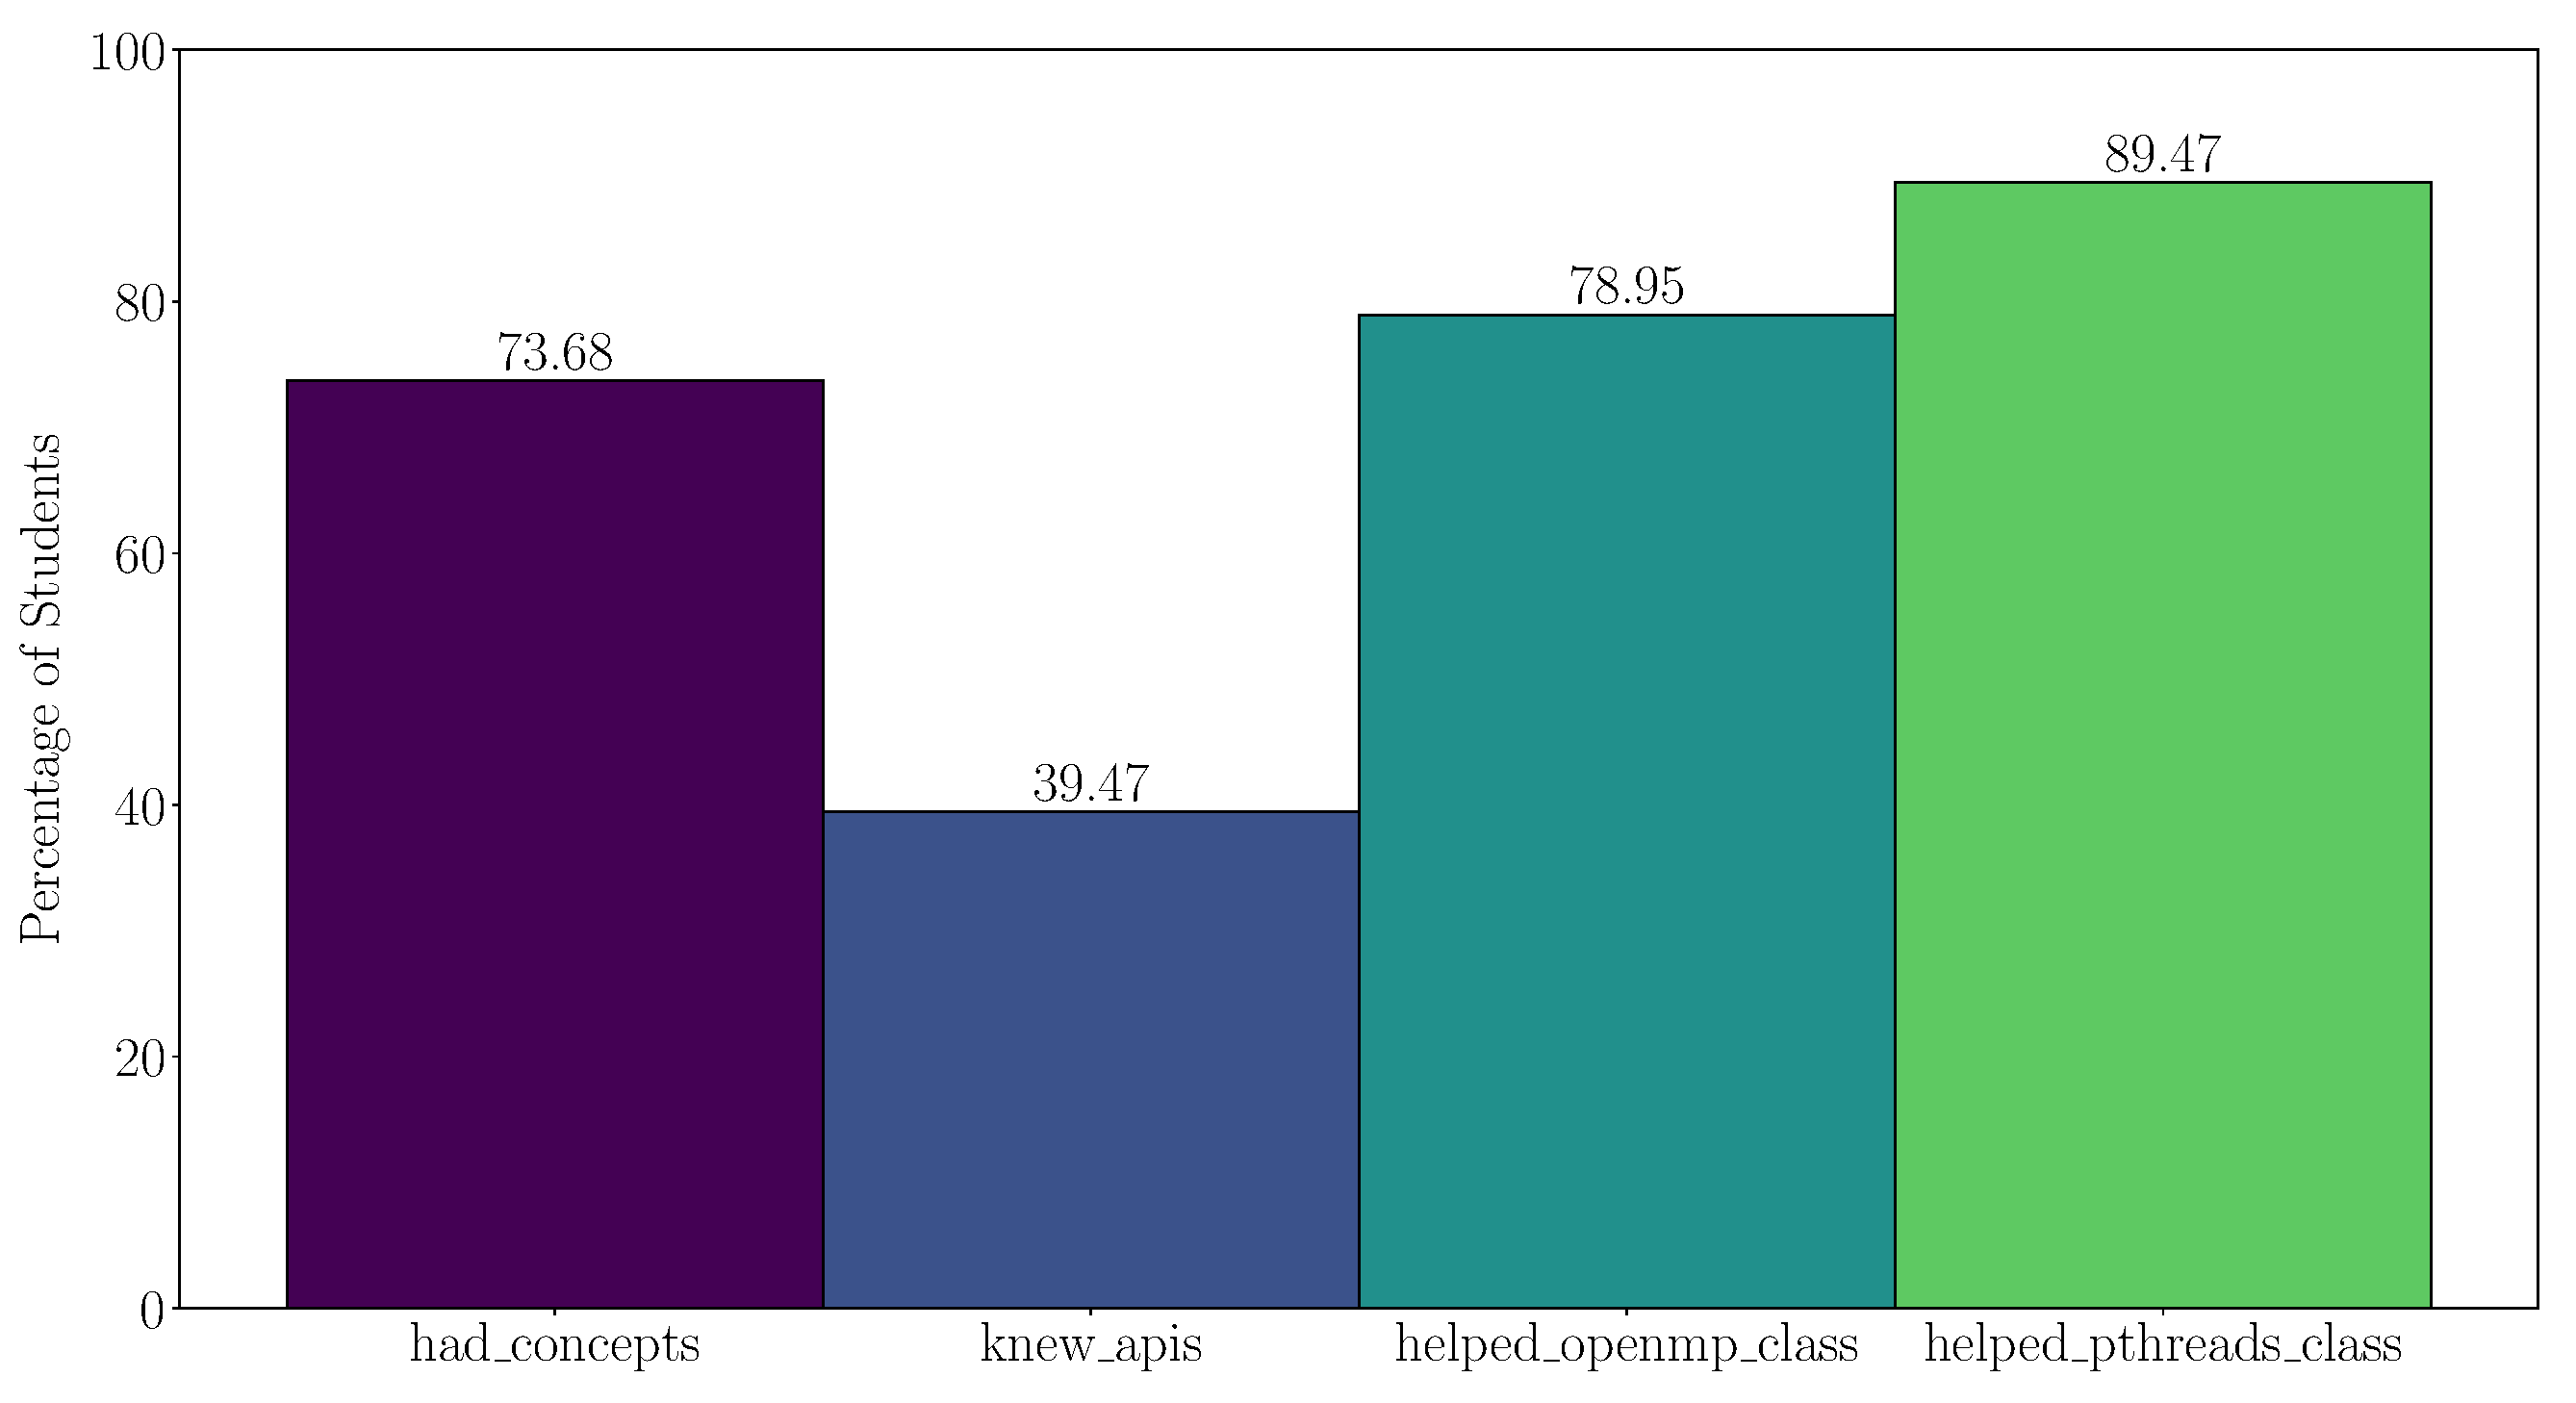
\includegraphics[width=0.85\columnwidth]{yes_no_questions}
    \caption{Student API knowledge \textit{before} the assignment and their relation to classes}
    \label{fig:student-knowledge-yes-no}
\end{figure}



\section{Results}
\label{sec:results}

\begin{figure}[htpb]
    \centering
    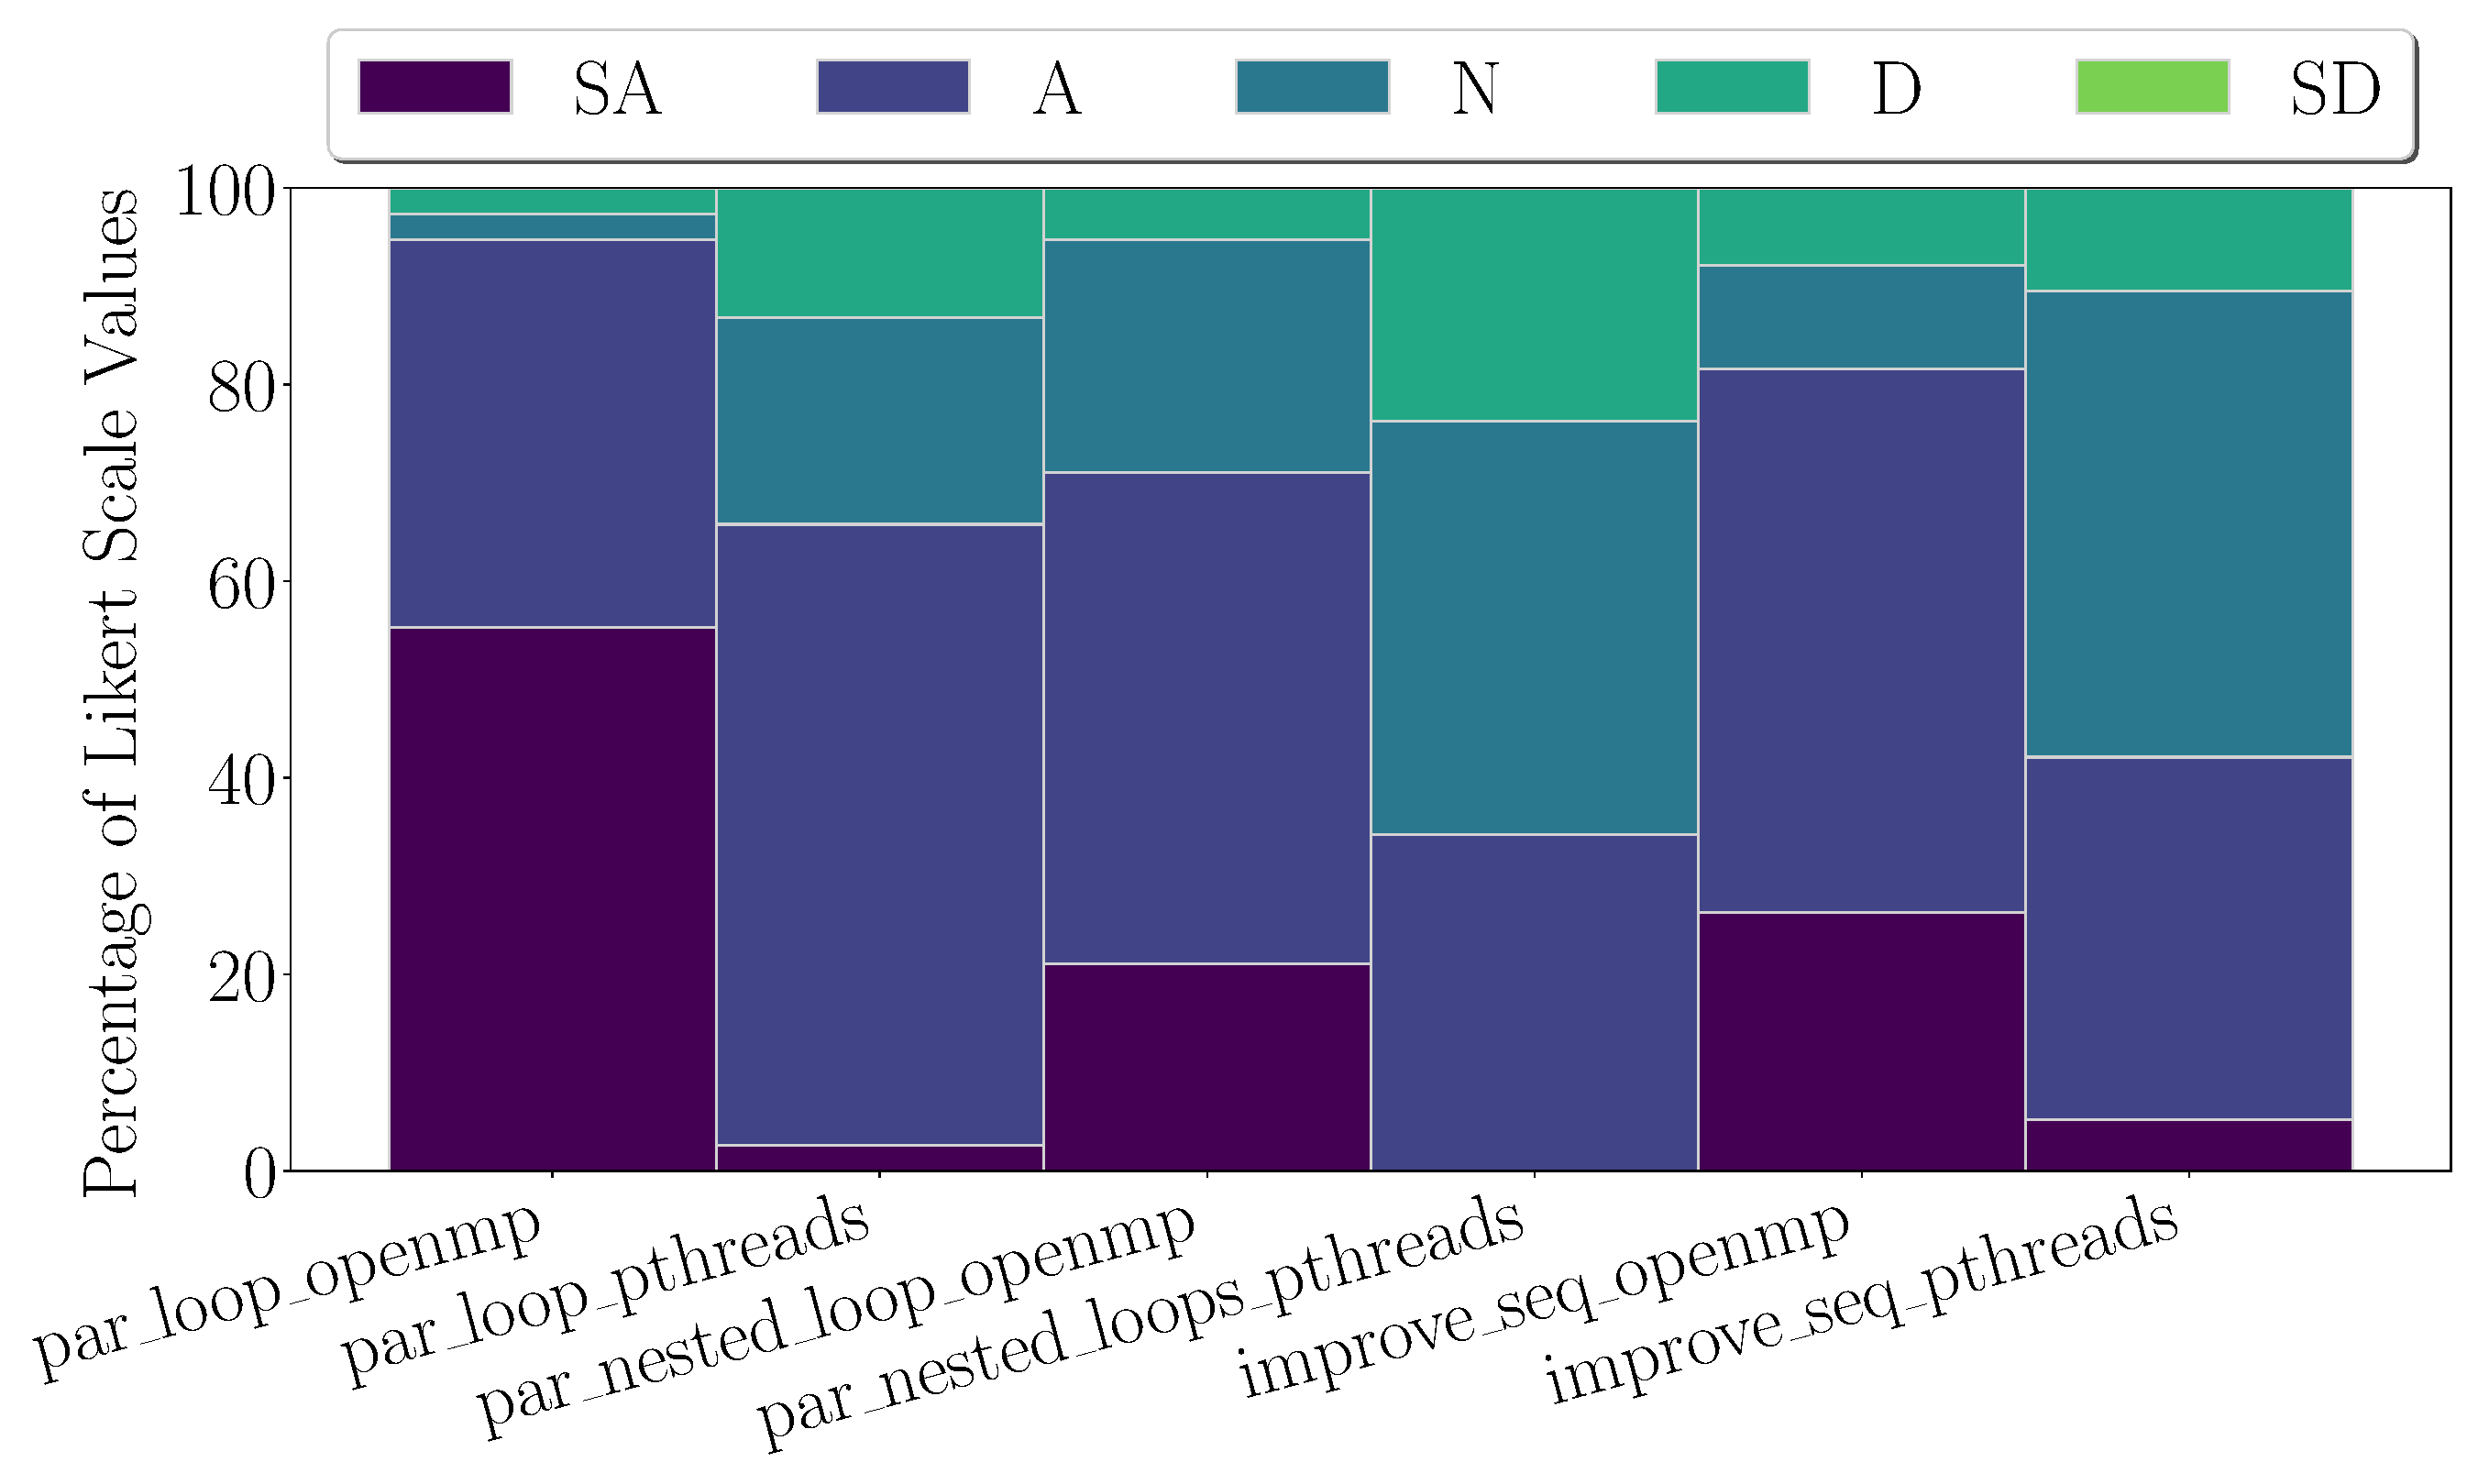
\includegraphics[width=0.85\columnwidth]{likert_questions}
    \caption{Student responses to Likert-scale questions}
    \label{fig:}
\end{figure}

\begin{figure}[htpb]
    \centering
    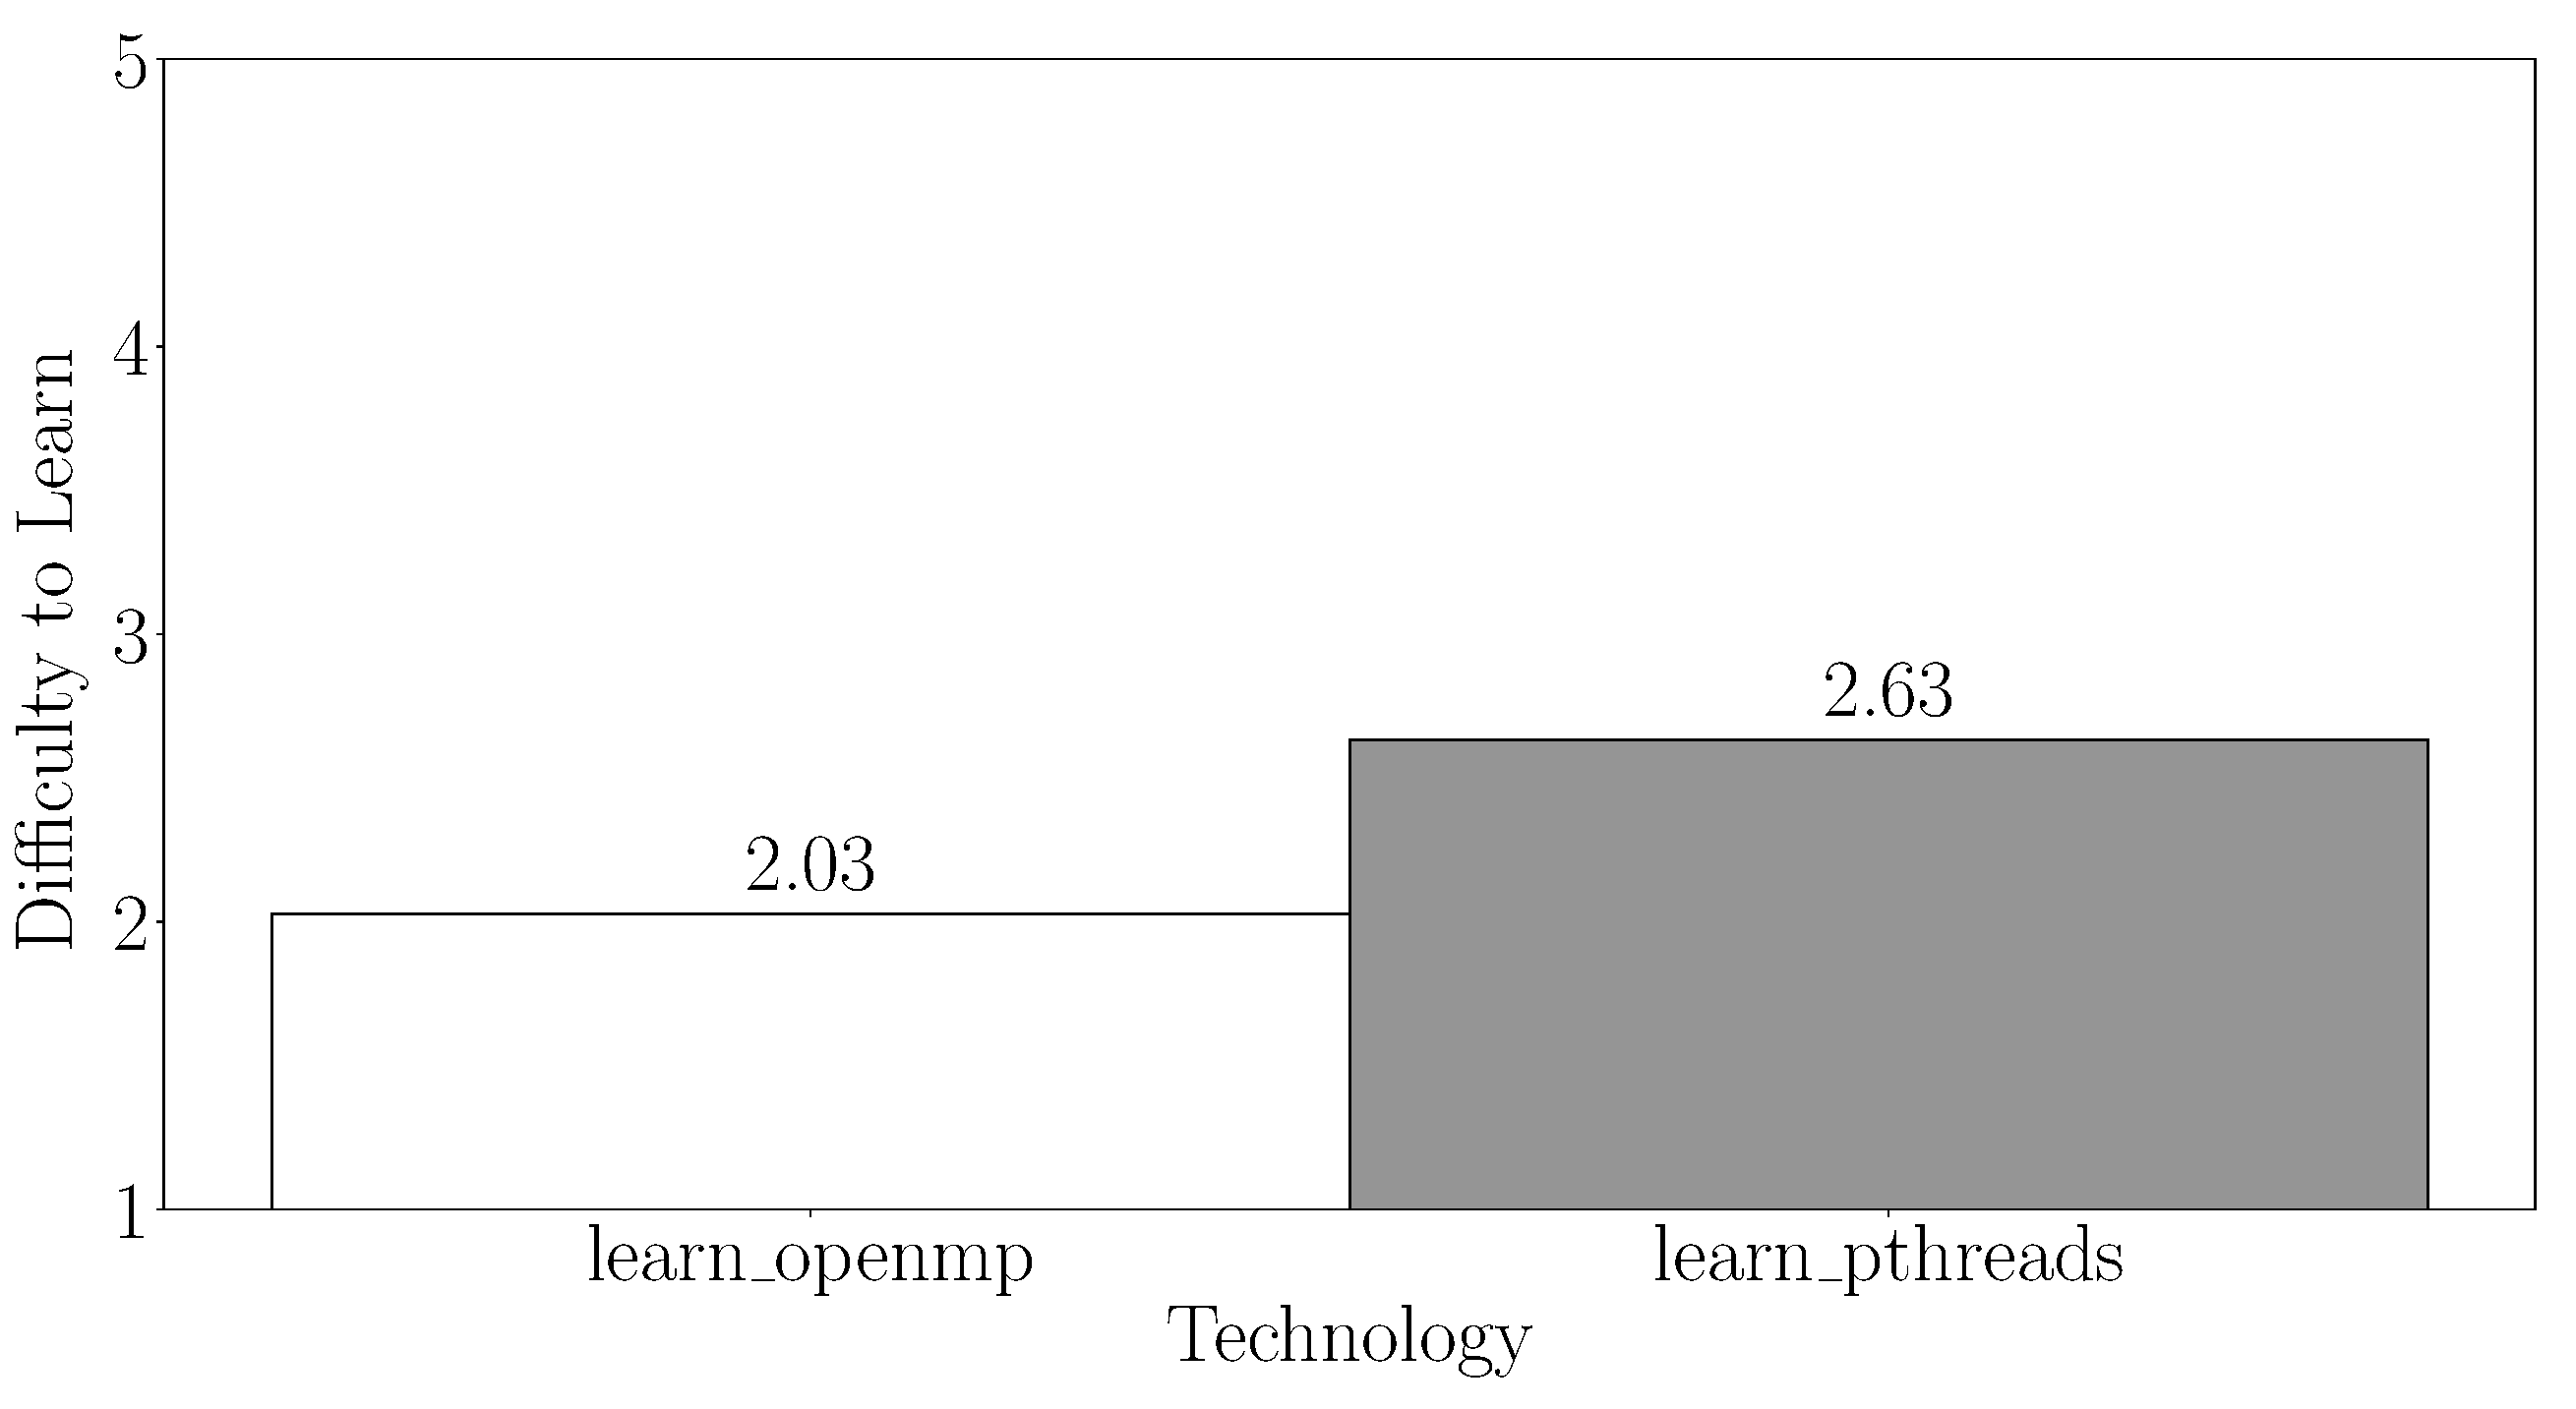
\includegraphics[width=0.85\columnwidth]{learning_mean_difficulty}
    \caption{Student mean difficulty to learn the APIs}
    \label{fig:}
\end{figure}

\begin{figure}[htpb]
    \centering
    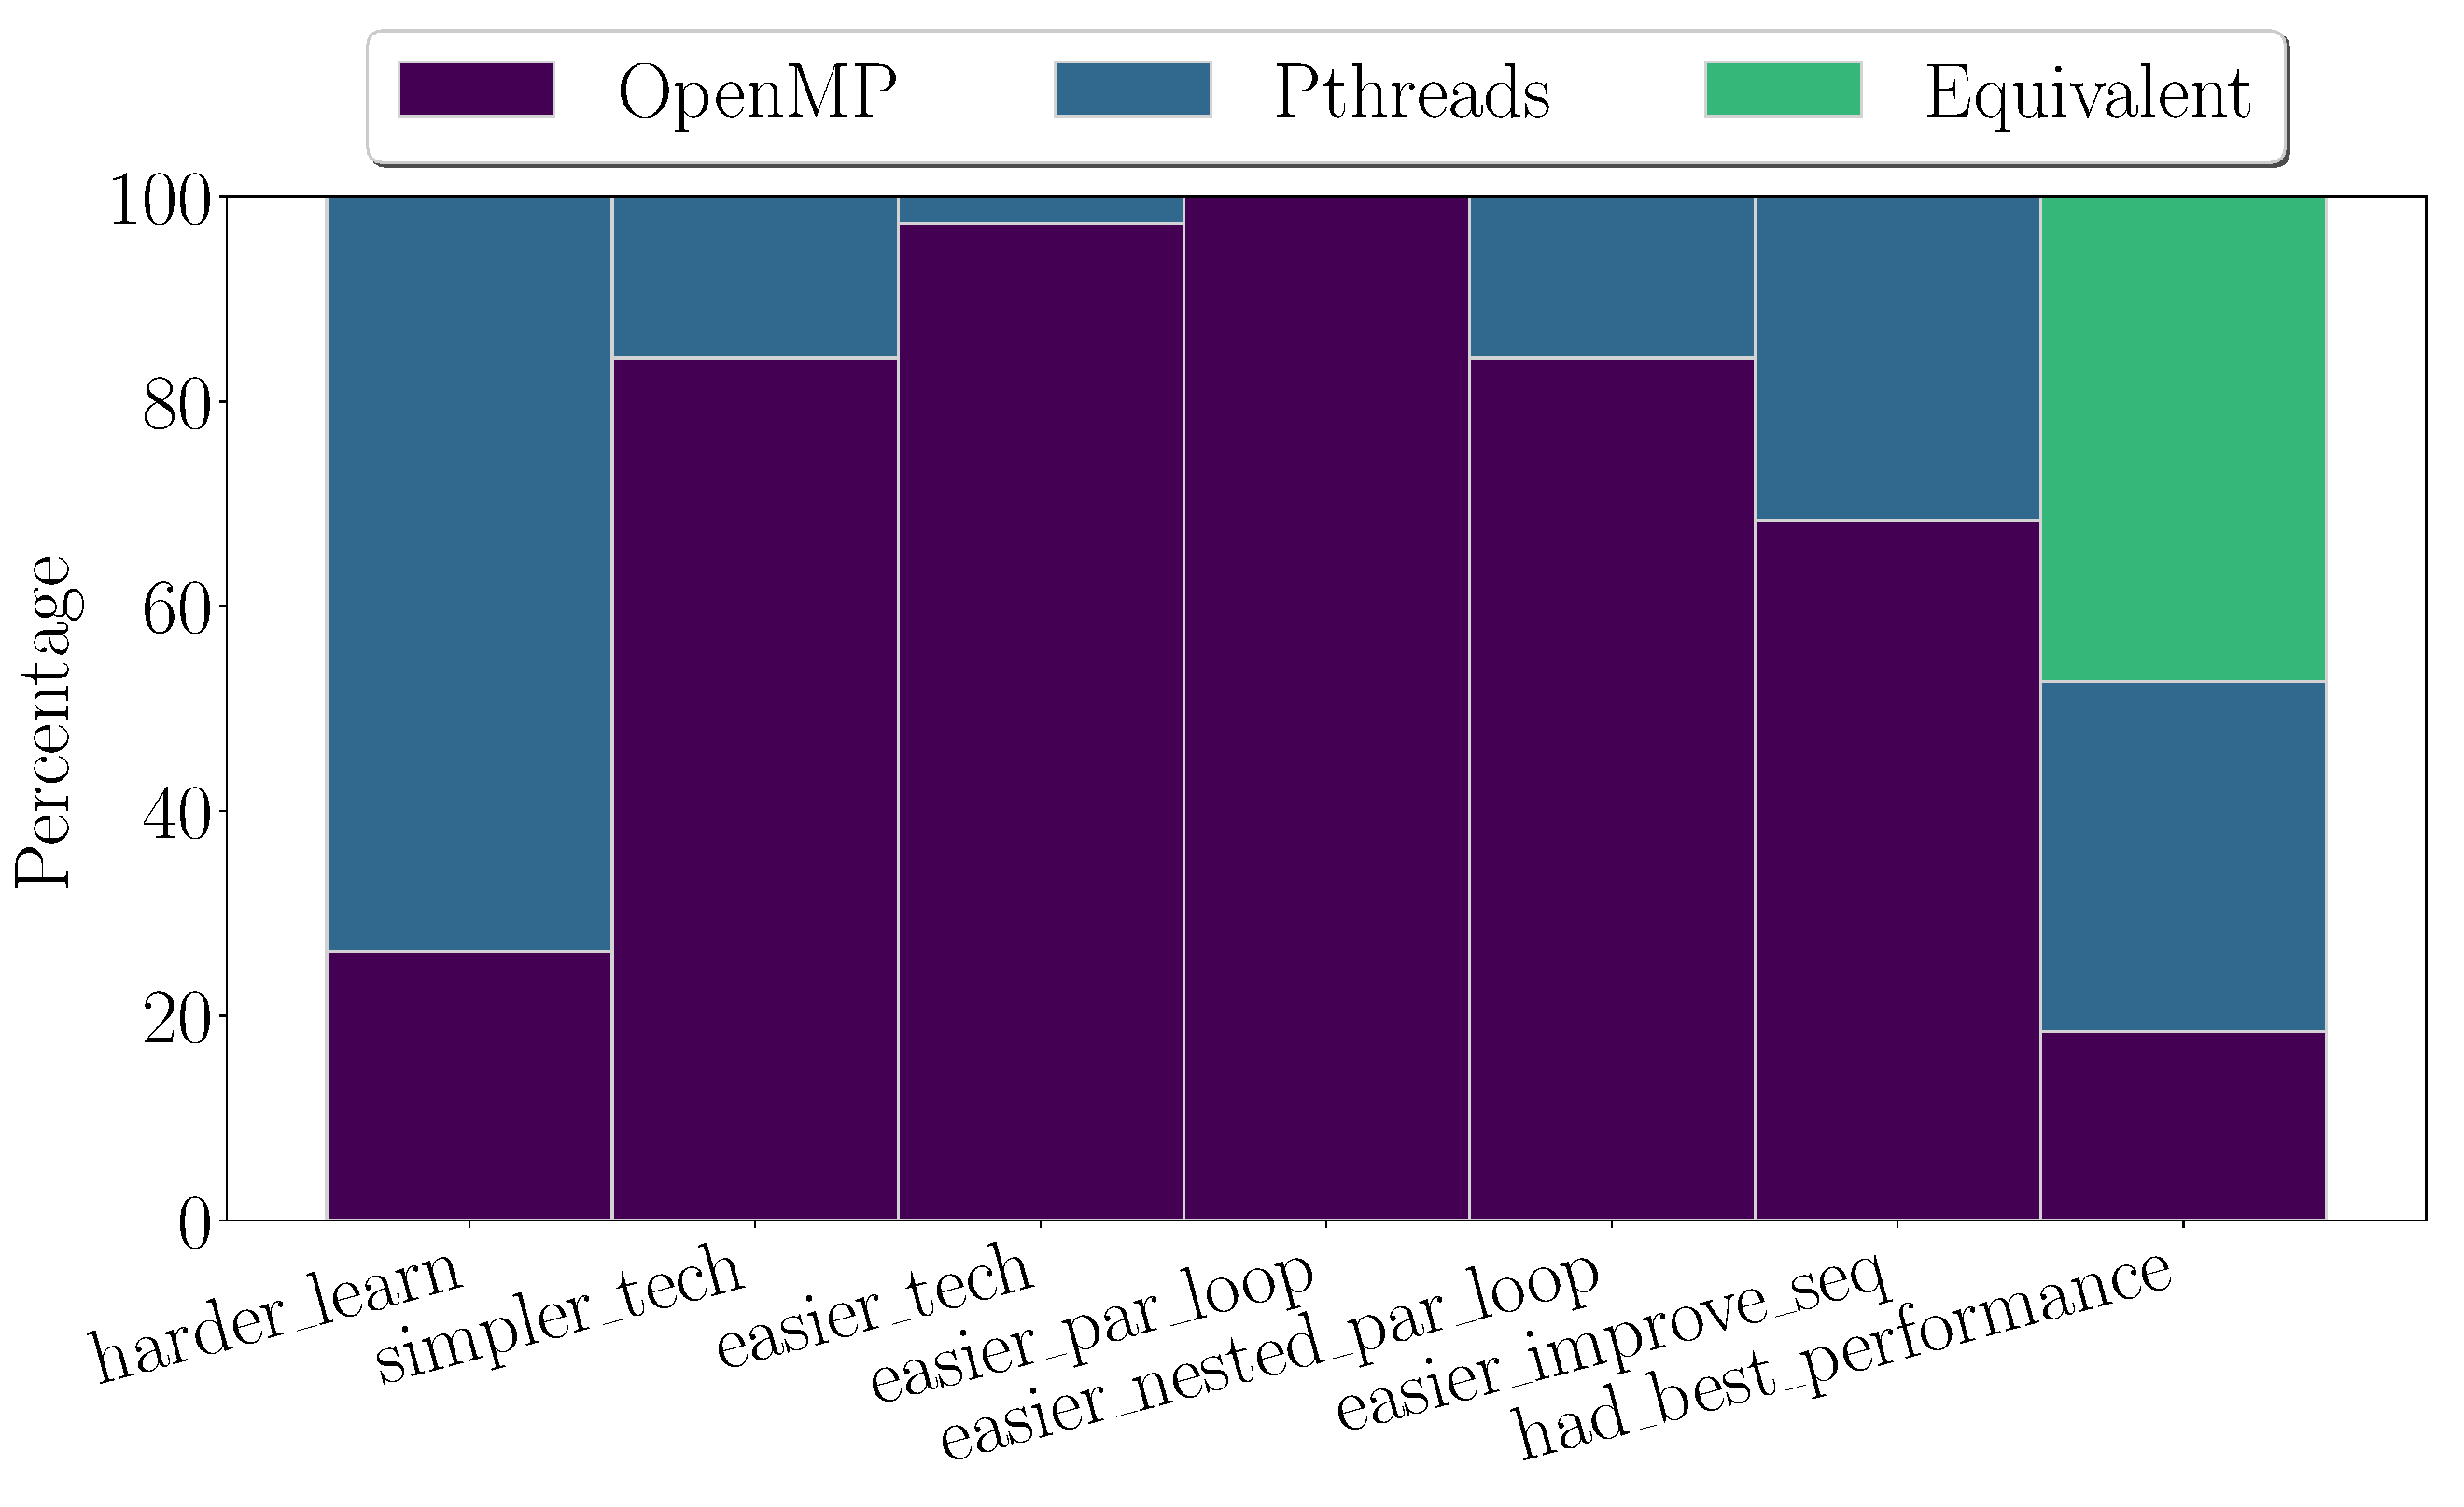
\includegraphics[width=0.85\columnwidth]{comparisons}
    \caption{Student responses on comparisons of APIs, and the performance of their usage of the APIs}
    \label{fig:}
\end{figure}


\section{Lessons Learned}
\label{sec:lessons}

TO-DO ...

\section{Conclusions}
\label{sec:conclusions}

TO-DO ...

%---
\section*{Acknowledgments}
\label{sec:acknowledgments}

The authors would like to thank Students who participated in this exercise ...


%---

\bibliographystyle{ACM-Reference-Format}
\bibliography{seps-omp-paper}

\end{document}
